\documentclass[12pt,a4paper]{article}

\usepackage[utf8]{inputenc}
\usepackage[T1]{fontenc}
\IfFileExists{indonesian.ldf}{\usepackage[indonesian]{babel}}{\usepackage[main=indonesian,provide=*]{babel}}
\usepackage{mathptmx}
\usepackage[a4paper,top=2.5cm,bottom=2.5cm,left=3cm,right=2.5cm]{geometry}
\usepackage{amsmath,amssymb}
\usepackage{graphicx}
\usepackage{booktabs,array,longtable}
\usepackage{listings}
\usepackage{xcolor}
\usepackage{fancyhdr}
\usepackage{enumitem}
\usepackage{caption}
\usepackage{float}
\usepackage{setspace}
\usepackage{microtype}
\usepackage{tikz}
\usetikzlibrary{arrows.meta,positioning,shapes.geometric,fit}
\usepackage[hidelinks]{hyperref}

\setstretch{1.15}
\setlength{\headheight}{14.5pt}
\setlength{\parindent}{1.0cm}
\setlength{\parskip}{3pt}
\setlength{\emergencystretch}{3em}
\setlist{itemsep=1pt,topsep=3pt}
\captionsetup{font=small,labelfont=bf}

\newcommand{\namakelompok}{Gerobak Pasar Kosambi}
\newcommand{\repourl}{https://github.com/i-Jer/Tubes1-Algeo-2026}

\lstdefinestyle{keluaran}{
  basicstyle=\ttfamily\scriptsize,
  frame=single, framerule=0.4pt, rulecolor=\color{black!40},
  backgroundcolor=\color{black!3},
  breaklines=true, columns=fullflexible, keepspaces=true,
  xleftmargin=0pt, aboveskip=6pt, belowskip=6pt
}
\lstset{style=keluaran}

\pagestyle{fancy}
\fancyhf{}
\fancyhead[L]{\small Kelompok \namakelompok}
\fancyhead[R]{\small IF2123 Aljabar Linier dan Geometri}
\fancyfoot[C]{\small\thepage}
\renewcommand{\headrulewidth}{0.4pt}
\fancypagestyle{plain}{\fancyhf{}\fancyfoot[C]{\small\thepage}\renewcommand{\headrulewidth}{0pt}}

\newcommand{\mat}[1]{\mathbf{#1}}
\DeclareMathOperator{\adj}{adj}
\DeclareMathOperator{\sgn}{sgn}

\begin{document}

\begin{titlepage}
  \centering
  \vspace*{0.5cm}
  {\large\bfseries LAPORAN TUGAS BESAR 1\par}
  \vspace{0.3cm}
  {\large IF2123 Aljabar Linier dan Geometri\par}
  \vspace{0.6cm}
  {\Large\bfseries Pustaka Aljabar Linier dalam Java:\\[2pt]
  Sistem Persamaan Linier, Determinan, Matriks Balikan,\\[2pt]
  Interpolasi, dan Regresi Spline\par}
  \vspace{0.6cm}
  {\large Kelompok \namakelompok\par}
  \vspace{0.8cm}

  \IfFileExists{foto-kelompok.jpg}{
\includegraphics[width=0.62\textwidth]{foto-kelompok.jpg}\par}{}
  \vspace{0.8cm}

  {\bfseries Anggota Kelompok\par}
  \vspace{0.2cm}
  \begin{tabular}{@{}ll@{}}
    Jeremy Gerald Sutanto & 13525104 \\
    Christian Immanuel & 13525116 \\
    Denzel Santoso & 13525014 \\
  \end{tabular}

  \vfill
  {\large Program Studi Teknik Informatika\\
  Sekolah Teknik Elektro dan Informatika\\
  Institut Teknologi Bandung\\[2pt]
  Semester I Tahun 2026/2027\par}
\end{titlepage}

\pagenumbering{roman}
\tableofcontents
\clearpage
\pagenumbering{arabic}

\section{Pendahuluan}

\subsection{Deskripsi Masalah}
Dalam skenario tugas besar ini, seorang peneliti muda bernama Mitya memimpin eksperimen berskala raksasa bernama Proyek Stuzha di Teyvat. Perhitungan berdimensi tinggi yang diperlukan proyek tersebut tidak lagi dapat ditangani oleh kalkulator saku miliknya yang sering \textit{error}. Kelompok kami ditugaskan membangun perangkat lunak sekelas \textit{Photomath} versi Teyvat, yaitu mesin kalkulasi otomatis yang mampu melumat sistem matriks dan persamaan linier yang rumit.

\subsection{Latar Belakang}
Aljabar linier adalah fondasi komputasi modern yang menggerakkan simulasi rekayasa, pemodelan aliran energi, analisis data, hingga dinamika sistem kompleks. Agar kalkulasi Proyek Stuzha tidak runtuh di tengah jalan, kami ditugaskan merancang dan membangun pustaka (\textit{library}) komputasi aljabar linier mandiri berbasis bahasa pemrograman Java yang modular, tangguh, dan terdokumentasi rapi. Pustaka ini menjadi mesin utama alat komputasi Mitya untuk:
\begin{itemize}
  \item menyelesaikan sistem persamaan linier (SPL), menghitung determinan, dan mencari matriks balikan guna menganalisis keseimbangan sirkuit daya dan kestabilan instrumen;
  \item melakukan interpolasi polinomial, \textit{natural cubic spline interpolation}, dan regresi \textit{spline} untuk memetakan jalur transfer energi serta memodelkan kontur data eksperimen secara presisi.
\end{itemize}

\subsection{Tujuan}
\begin{enumerate}
  \item Mengimplementasikan metode penyelesaian SPL, determinan, matriks balikan, interpolasi polinomial, \textit{natural cubic spline interpolation}, dan regresi \textit{spline} secara mandiri menggunakan Java.
  \item Membangun pustaka aljabar linier yang terstruktur secara modular, bersih, dan terdokumentasi dengan baik tanpa memakai pustaka perhitungan matriks, regresi, atau interpolasi instan.
  \item Menguji keandalan pustaka pada berbagai kasus uji analitis, serta menyusun laporan analisis hasil perhitungannya.
\end{enumerate}

\section{Dasar Teori}

\subsection{Sistem Persamaan Linier}
Sistem persamaan linier (SPL) dengan $m$ persamaan dan $n$ variabel dapat ditulis sebagai $A\mat{x}=\mat{b}$ dengan $A\in\mathbb{R}^{m\times n}$, atau dalam bentuk matriks \textit{augmented} $[A\mid\mat{b}]$. Solusi SPL dapat berupa solusi tunggal, tak hingga banyak solusi, atau tidak ada solusi \cite{anton}.

\subsubsection{Eliminasi Gauss}
Matriks \textit{augmented} diubah menjadi matriks eselon baris menggunakan operasi baris elementer (OBE): menukar dua baris, mengalikan baris dengan skalar tak nol, dan menambahkan kelipatan suatu baris ke baris lain. Solusi diperoleh dengan substitusi mundur. Untuk menjaga stabilitas numerik dipakai \textit{partial pivoting}, yaitu pada kolom ke-$k$ dipilih baris dengan $|a_{ik}|$ terbesar sebagai pivot sehingga pengali baris selalu bernilai $|l_{ik}|\le 1$.
Setelah eliminasi, SPL tidak memiliki solusi jika terdapat baris berbentuk $[0\ \cdots\ 0\mid c]$ dengan $c\neq 0$. Jika tidak, banyaknya variabel bebas sama dengan $n-\operatorname{rank}(A)$; bila nol maka solusi tunggal, selain itu solusi berbentuk parametrik.

\subsubsection{Eliminasi Gauss-Jordan}
Eliminasi dilanjutkan hingga diperoleh matriks eselon baris tereduksi: setiap pivot bernilai 1 dan merupakan satu-satunya elemen tak nol pada kolomnya. Solusi dapat dibaca langsung tanpa substitusi mundur yang panjang.

\subsubsection{Metode Matriks Balikan}
Jika $A$ persegi dan $\det(A)\neq0$, maka $A\mat{x}=\mat{b}$ memiliki solusi tunggal $\mat{x}=A^{-1}\mat{b}$.

\subsubsection{Kaidah Cramer}
Untuk SPL persegi dengan $\det(A)\neq 0$, solusi tunggalnya adalah
\begin{equation}
  x_i=\frac{\det(A_i)}{\det(A)},\qquad i=1,\dots,n,
\end{equation}
dengan $A_i$ adalah matriks $A$ yang kolom ke-$i$-nya diganti $\mat{b}$.

\subsection{Determinan Matriks}
Determinan $\det(A)$ hanya terdefinisi untuk matriks persegi dan menentukan apakah matriks memiliki balikan ($\det(A)\ne0$).

\paragraph{Reduksi baris (OBE).} Matriks direduksi menjadi segitiga atas. Menambahkan kelipatan satu baris ke baris lain tidak mengubah determinan, setiap pertukaran baris mengalikan determinan dengan $-1$, dan mengalikan satu baris dengan $k$ mengalikan determinan dengan $k$. Bila $s$ adalah banyaknya pertukaran baris dan $u_{ii}$ elemen diagonal hasil reduksi, maka
\begin{equation}
  \det(A)=(-1)^{s}\prod_{i=1}^{n}u_{ii}.
\end{equation}

\paragraph{Ekspansi kofaktor.} Untuk sembarang baris $i$ (atau kolom $j$),
\begin{equation}
  \det(A)=\sum_{j=1}^{n}a_{ij}C_{ij},\qquad C_{ij}=(-1)^{i+j}M_{ij},
\end{equation}
dengan $M_{ij}$ determinan submatriks hasil penghapusan baris $i$ dan kolom $j$. Pemilihan baris atau kolom yang memuat banyak nol mengurangi jumlah suku yang harus dihitung. Kompleksitas metode ini $O(n!)$ sehingga hanya praktis untuk matriks kecil, sedangkan reduksi baris berkompleksitas $O(n^3)$.

\subsection{Matriks Balikan}
Matriks persegi $A$ memiliki balikan $A^{-1}$ dengan $AA^{-1}=A^{-1}A=I$ jika dan hanya jika $\det(A)\neq0$.

\paragraph{Metode augmentasi $[A\mid I]$.} Matriks $[A\mid I]$ direduksi dengan eliminasi Gauss-Jordan menjadi $[I\mid A^{-1}]$.

\paragraph{Metode adjoin.}
\begin{equation}
  A^{-1}=\frac{1}{\det(A)}\adj(A),\qquad \adj(A)=C^{T},
\end{equation}
dengan $C$ matriks kofaktor, $C_{ij}=(-1)^{i+j}\det(M_{ij})$.

\subsection{Interpolasi Polinomial}
Diberikan $n$ titik berbeda $(x_i,y_i)$, terdapat tepat satu polinom berderajat paling tinggi $n-1$,
$P(x)=a_0+a_1x+\dots+a_{n-1}x^{n-1}$, yang melalui seluruh titik tersebut \cite{burden}. Koefisien diperoleh dengan menyelesaikan SPL Vandermonde
\begin{equation}
  \begin{bmatrix}
    1 & x_1 & \cdots & x_1^{n-1}\\
    \vdots & \vdots & & \vdots\\
    1 & x_n & \cdots & x_n^{n-1}
  \end{bmatrix}
  \begin{bmatrix}a_0\\ \vdots\\ a_{n-1}\end{bmatrix}
  =
  \begin{bmatrix}y_1\\ \vdots\\ y_n\end{bmatrix}.
\end{equation}
Polinom ini dapat dipakai untuk interpolasi (di dalam $[x_{\min},x_{\max}]$) maupun ekstrapolasi. Matriks Vandermonde berkondisi buruk bila $n$ besar, sehingga galat pembulatan dapat membesar.

\subsection{Natural Cubic Spline Interpolation}
Interpolasi polinomial berderajat tinggi rentan berosilasi liar. \textit{Cubic spline} menghindarinya dengan memakai potongan polinom kubik $S_j(x)$ pada tiap subinterval $[x_j,x_{j+1}]$, $j=0,\dots,n-2$ untuk $n$ titik, dengan syarat $S$ melalui semua titik serta $S$, $S'$, dan $S''$ kontinu di setiap simpul dalam \cite{burden,deboor}. Pada \textit{natural spline} ditambahkan syarat batas $S''(x_0)=S''(x_{n-1})=0$.

Bila $M_j=S''(x_j)$ dan $h_j=x_{j+1}-x_j$, maka tiap segmen berbentuk
\begin{equation}
  S_j(x)=a_j+b_j(x-x_j)+c_j(x-x_j)^2+d_j(x-x_j)^3,
\end{equation}
dengan
\begin{equation}
  a_j=y_j,\quad
  b_j=\frac{y_{j+1}-y_j}{h_j}-\frac{h_j(2M_j+M_{j+1})}{6},\quad
  c_j=\frac{M_j}{2},\quad
  d_j=\frac{M_{j+1}-M_j}{6h_j}.
\end{equation}
Kekontinuan turunan pertama di simpul dalam menghasilkan SPL \textbf{tridiagonal} untuk $M_1,\dots,M_{n-2}$:
\begin{equation}
  h_{i-1}M_{i-1}+2(h_{i-1}+h_i)M_i+h_iM_{i+1}
  =6\left(\frac{y_{i+1}-y_i}{h_i}-\frac{y_i-y_{i-1}}{h_{i-1}}\right),
  \quad i=1,\dots,n-2,
\end{equation}
dengan syarat batas natural $M_0=M_{n-1}=0$. Matriks koefisiennya dominan secara diagonal ($2(h_{i-1}+h_i)>h_{i-1}+h_i$) sehingga selalu non-singular dan solusi $M_i$ tunggal.

\subsection{Regresi Spline Kubik}
Berbeda dengan interpolasi, regresi \textit{spline} tidak mengharuskan kurva melalui setiap titik, tetapi meminimalkan jumlah kuadrat galat terhadap $N$ data pengamatan \cite{hastie,james}. Untuk $K$ simpul (\textit{knot}) $\xi_1<\dots<\xi_K$, ruang \textit{spline} kubik berdimensi $M=4+K$ dengan \textit{truncated power basis}
\begin{equation}
  h_0=1,\ h_1=x,\ h_2=x^2,\ h_3=x^3,\qquad h_{3+k}(x)=(x-\xi_k)_+^3,
\end{equation}
dengan $(u)_+=\max(0,u)$. Fungsi regresi adalah $\hat y(x)=\sum_{j=0}^{3+K}\beta_jh_j(x)$, yang otomatis kontinu hingga turunan kedua ($C^2$). Dengan matriks desain $X\in\mathbb{R}^{N\times M}$, $X_{ij}=h_j(x_i)$, masalah $X\boldsymbol\beta\approx\mathbf{y}$ bersifat \textit{overdetermined} ($N>M$). Solusi kuadrat terkecil diperoleh dari proyeksi ortogonal $\mathbf{y}$ ke $\operatorname{Col}(X)$, yaitu persamaan normal
\begin{equation}
  (X^{T}X)\hat{\boldsymbol\beta}=X^{T}\mathbf{y}.
\end{equation}
Jika kolom-kolom $X$ bebas linier maka $X^TX$ non-singular dan $\hat{\boldsymbol\beta}=(X^TX)^{-1}X^T\mathbf{y}$ tunggal. Persamaan normal ini adalah SPL berukuran $M\times M$ yang diselesaikan dengan eliminasi Gauss.

\section{Implementasi}

Seluruh pustaka dan program ditulis dalam Java (target Java 17) tanpa pustaka eksternal untuk perhitungan matriks. Pustaka hanya memakai \texttt{java.lang.Math} untuk fungsi dasar (\texttt{abs}, \texttt{max}, \texttt{round}) dan kelas standar Java untuk berkas dan masukan (\texttt{java.io}, \texttt{java.util}).

\subsection{Struktur Kelas}
Kode sumber berada di \texttt{src/main/java/algeo} dan dibagi ke dalam paket-paket berikut.

{\small\renewcommand{\arraystretch}{1.2}
\begin{longtable}{@{}p{2.7cm}p{3.3cm}p{8.2cm}@{}}
\caption{Paket dan kelas pada program}\\
\toprule
\textbf{Paket} & \textbf{Kelas} & \textbf{Tanggung jawab dan metode penting}\\
\midrule\endfirsthead
\toprule
\textbf{Paket} & \textbf{Kelas} & \textbf{Tanggung jawab dan metode penting}\\
\midrule\endhead
\texttt{matrix} & \texttt{Matrix} &
 Struktur data matriks (atribut \texttt{rows}, \texttt{cols}, \texttt{double[][] data}). OBE: \texttt{swapRows}, \texttt{multiplyRow}, \texttt{addRowMultiple}. Operasi: \texttt{add}, \texttt{subtract}, \texttt{multiply} (skalar dan matriks), \texttt{transpose}, \texttt{submatrix}, \texttt{slice}, \texttt{augment}, \texttt{identity}, \texttt{copy}. Pemformatan: \texttt{round3}, \texttt{formatNumber}.\\
\addlinespace
\texttt{spl} & \texttt{Elimination} &
 \texttt{toRowEchelonForm} dan \texttt{toReducedRowEchelonForm} dengan \textit{partial pivoting}; mencatat langkah OBE; \texttt{tolerance} untuk deteksi nol.\\
 & \texttt{SPLSolver} &
 \texttt{gauss}, \texttt{gaussJordan}, \texttt{inverseMethod}, \texttt{cramer}; \textit{substitusi mundur} dan penentuan jenis solusi.\\
 & \texttt{SPLResult} &
 Hasil SPL: jenis (\texttt{UNIQUE}, \texttt{NONE}, \texttt{INFINITE}) dan ekspresi tiap variabel $x_i=c+\sum_k a_kt_k$.\\
\addlinespace
\texttt{determinant} & \texttt{Determinant} &
 \texttt{byRowReduction} (OBE) dan \texttt{byCofactorExpansion} (memilih baris/kolom dengan nol terbanyak).\\
\texttt{inverse} & \texttt{Inverse} &
 \texttt{byGaussJordan} (augmentasi $[A\mid I]$) dan \texttt{byAdjoint}.\\
\texttt{interpolasi} & \texttt{Interpolasi} &
 \texttt{calculateCoefficient} (SPL Vandermonde), \texttt{evaluator} (skema Horner), \texttt{toEquation}.\\
 & \texttt{NaturalCubicSpline} &
 Membangun SPL tridiagonal untuk $M_i$, koefisien $a_j,b_j,c_j,d_j$, \texttt{evaluate}, \texttt{toString}.\\
\texttt{regression} & \texttt{SplineRegression} &
 Basis \textit{truncated power}, matriks desain $X$, persamaan normal, \texttt{predict}, \texttt{toEquation}.\\
\addlinespace
\texttt{io} & \texttt{FileIO} &
 Membaca matriks/titik dari \texttt{.txt}, \texttt{parseNumber} (menerima titik atau koma desimal), menulis hasil.\\
 & \texttt{ConsoleInput} &
 Masukan \textit{keyboard} yang tervalidasi (bilangan bulat berbatas, angka, y/n).\\
 & \texttt{Style}, \texttt{InputEnd\-Exception} &
 Tampilan CLI (menu, banner, warna, mode \texttt{--plain}) dan penanda berakhirnya masukan.\\
\texttt{cli} & \texttt{CLI} &
 Menu utama, submenu metode, pembacaan masukan, penyusunan laporan, dan penyimpanan hasil.\\
(akar) & \texttt{App} & Titik masuk program (\texttt{main}).\\
\bottomrule
\end{longtable}}

\subsection{Arsitektur Pustaka}
Pustaka disusun berlapis: lapisan terbawah adalah \texttt{Matrix}; di atasnya \texttt{Elimination} menyediakan eliminasi baris yang dipakai bersama oleh seluruh modul. Modul interpolasi dan regresi tidak menulis penyelesai sendiri, melainkan menyusun SPL lalu memanggil \texttt{SPLSolver.gauss}. Lapisan \texttt{cli} dan \texttt{io} hanya berinteraksi dengan pengguna dan tidak berisi logika matematika.

\begin{figure}[H]
\centering
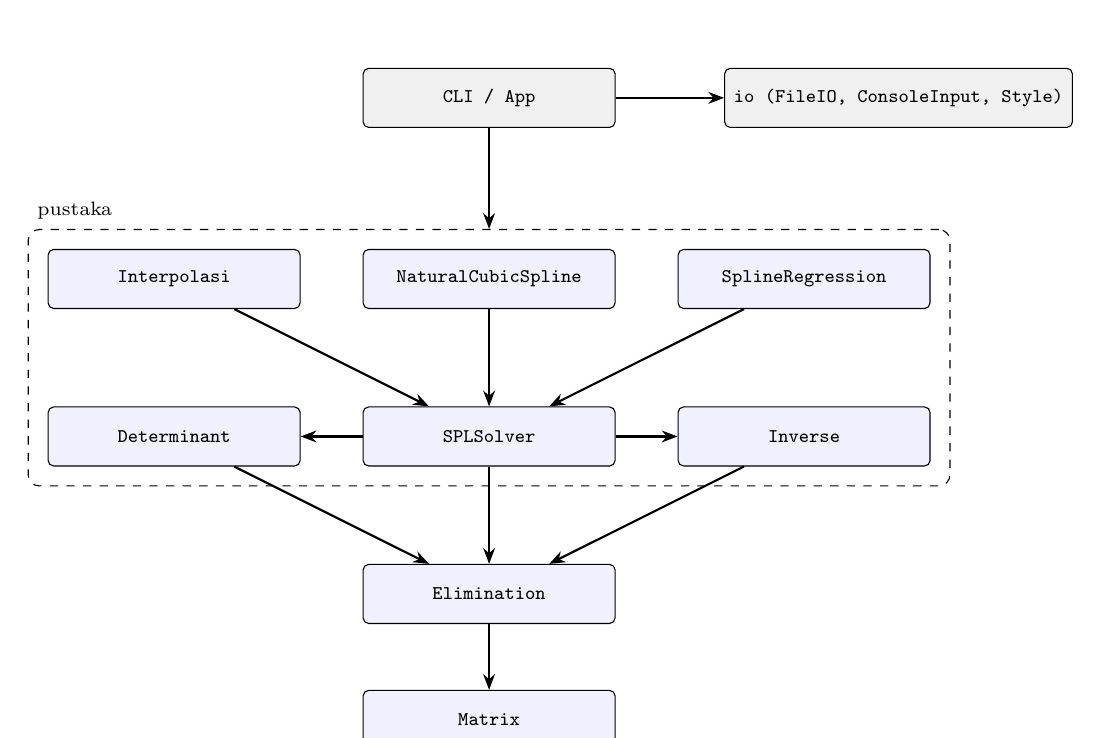
\begin{tikzpicture}[
  box/.style={draw,rounded corners=2pt,minimum height=0.75cm,minimum width=3.2cm,align=center,font=\scriptsize\ttfamily,fill=blue!6},
  top/.style={box,fill=black!6},
  ar/.style={-{Stealth[length=2mm]},thick}]
  \node[top] (cli) at (0,0) {CLI / App};
  \node[top] (io)  at (5.2,0) {io (FileIO, ConsoleInput, Style)};
  \node[box] (itp) at (-4,-2.3) {Interpolasi};
  \node[box] (ncs) at (0,-2.3) {NaturalCubicSpline};
  \node[box] (reg) at (4,-2.3) {SplineRegression};
  \node[box] (det) at (-4,-4.3) {Determinant};
  \node[box] (spl) at (0,-4.3) {SPLSolver};
  \node[box] (inv) at (4,-4.3) {Inverse};
  \node[box] (elim) at (0,-6.3) {Elimination};
  \node[box] (mat) at (0,-7.9) {Matrix};
  \node[draw,dashed,rounded corners=4pt,inner sep=7pt,fit=(itp)(reg)(inv)(det),label={[font=\scriptsize,anchor=south west]north west:pustaka}] (lib) {};
  \draw[ar] (cli) -- (io);
  \draw[ar] (cli) -- (lib.north -| cli);
  \draw[ar] (itp) -- (spl);
  \draw[ar] (ncs) -- (spl);
  \draw[ar] (reg) -- (spl);
  \draw[ar] (spl) -- (det);
  \draw[ar] (spl) -- (inv);
  \draw[ar] (det) -- (elim);
  \draw[ar] (spl) -- (elim);
  \draw[ar] (inv) -- (elim);
  \draw[ar] (elim) -- (mat);
\end{tikzpicture}
\caption{Ketergantungan antarmodul (panah: ``memakai''). \texttt{SPLSolver} memakai \texttt{Determinant} (Kaidah Cramer) dan \texttt{Inverse} (metode balikan); \texttt{Inverse} juga memakai \texttt{Determinant} (metode adjoin)}
\end{figure}

\subsection{Rincian Algoritma}

\paragraph{Eliminasi dengan \textit{partial pivoting}.} Untuk tiap kolom, dicari baris pada/ di bawah baris pivot saat ini yang memiliki $|a_{ik}|$ terbesar lalu ditukar ke posisi pivot. Kolom dilewati jika pivot terbesar tidak lebih dari toleransi $\varepsilon=\max|a_{ij}|\cdot\max(m,n)\cdot10^{-15}$. Semua elemen di bawah pivot dinolkan, dan jumlah pertukaran baris dikembalikan agar dapat dipakai menghitung determinan. Gauss-Jordan melanjutkan dengan membagi baris pivot dan menolkan elemen di atas pivot.

\paragraph{Penentuan jenis solusi.} Setelah eliminasi, setiap baris diperiksa posisi elemen tak nolnya yang pertama. Bila posisi itu tepat di kolom konstanta, SPL tidak konsisten (\texttt{NONE}). Variabel tanpa pivot menjadi variabel bebas $t_1,t_2,\dots$; variabel berpivot dihitung dari baris terbawah ke atas dalam bentuk $c+\sum a_kt_k$ (substitusi mundur). Solusi tunggal berarti tidak ada variabel bebas. Bentuk parametrik dicetak sebagai, misalnya, $x_1 = 3.9 - 2t_1 - 2.9t_2$.

\paragraph{Determinan.} Metode OBE mereduksi salinan matriks ke segitiga atas, lalu mengalikan elemen diagonal dengan $(-1)^s$; bila ada diagonal bernilai nol (dalam toleransi) hasilnya $0$. Metode kofaktor bersifat rekursif dan pada tiap level memilih baris atau kolom dengan jumlah nol terbanyak, sehingga suku bernilai nol dilewati; dibatasi hingga $11\times11$.

\paragraph{Matriks balikan.} Metode augmentasi membentuk $[A\mid I]$ lalu mereduksinya dengan Gauss-Jordan; kesingularan diperiksa lebih dulu melalui reduksi baris. Metode adjoin menghitung seluruh kofaktor (determinan minor dengan reduksi baris), mentranspos menjadi $\adj(A)$, lalu mengalikannya dengan $1/\det(A)$. Metode balikan untuk SPL menghitung $\mat{x}=A^{-1}\mat{b}$ dan Kaidah Cramer menghitung $\det(A_i)/\det(A)$; keduanya hanya untuk SPL persegi.

\paragraph{Interpolasi polinomial.} Matriks Vandermonde disusun dari titik-titik masukan dan diselesaikan dengan \texttt{SPLSolver.gauss}; nilai $P(x_t)$ dihitung dengan skema Horner. Evaluasi hanya diizinkan di dalam domain $[x_{\min},x_{\max}]$.

\paragraph{Natural cubic spline.} Titik diurutkan menurut $x$ (pengurutan sisip), lalu $h_j$ dihitung dan SPL tridiagonal berukuran $(n-2)\times(n-2)$ dirakit dan diselesaikan dengan \texttt{SPLSolver.gauss}; $M_0=M_{n-1}=0$ diterapkan secara langsung. Koefisien tiap segmen dihitung dengan rumus pada Bab~2, dan evaluasi mencari segmen yang memuat $x_t$.

\paragraph{Regresi spline kubik.} Pengguna menentukan jumlah dan posisi \textit{knot}. Program menyusun matriks desain $X$ ($N\times(4+K)$) dengan \textit{truncated power basis}, menghitung $X^TX$ dan $X^T\mathbf{y}$ memakai operasi \texttt{Matrix}, lalu menyelesaikan persamaan normal dengan eliminasi Gauss. Program menolak masukan bila $N\le 4+K$ atau bila dua \textit{knot} sama.

\subsection{Alur Program}
\begin{enumerate}
  \item \texttt{App.main} menginisialisasi \texttt{Style} (opsi \texttt{--plain} mematikan warna/Unicode) lalu menjalankan \texttt{CLI.run}.
  \item \texttt{CLI} menampilkan \textbf{menu utama} (1.~SPL, 2.~Determinan, 3.~Matriks Balikan, 4.~Interpolasi Polinomial, 5.~\textit{Natural Cubic Spline}, 6.~Regresi Spline Kubik, 7.~Keluar). Menu 1, 2, 3, 4, dan 6 memiliki \textbf{submenu} pemilihan metode.
  \item Pengguna memilih sumber masukan: \textit{keyboard} (ukuran matriks dibatasi $11\times11$, atau $11\times12$ untuk \textit{augmented}; titik data maksimal 10) atau berkas \texttt{.txt} (matriks hingga $1001\times1001$, atau $1001\times1002$ untuk \textit{augmented}).
  \item Modul pustaka dipanggil dengan \texttt{StringBuilder} untuk mencatat langkah perhitungan (OBE, matriks antara, substitusi mundur, kofaktor, dan sebagainya). Untuk matriks yang lebih besar dari batas masukan \textit{keyboard}, langkah tidak dicatat agar keluaran tidak membanjiri layar.
  \item Laporan berisi metode, matriks/titik masukan, langkah, dan hasil ditampilkan di layar. Untuk interpolasi, \textit{spline}, dan regresi, program lalu meminta nilai $x$ berulang kali (kosongkan untuk selesai) untuk dievaluasi.
  \item Pengguna dapat menyimpan seluruh laporan ke berkas \texttt{.txt}; program kembali ke menu utama.
\end{enumerate}

\subsection{Penanganan Kesalahan}
Setiap kesalahan masukan atau komputasi ditangani dengan mekanisme \textit{exception} Java sehingga program tidak \textit{crash}.

\begin{table}[H]
\centering\small
\renewcommand{\arraystretch}{1.2}
\begin{tabular}{@{}p{4.6cm}p{4.4cm}p{4.6cm}@{}}
\toprule
\textbf{Situasi} & \textbf{Exception} & \textbf{Perilaku program}\\
\midrule
Karakter bukan angka pada masukan \textit{keyboard} atau berkas & \texttt{NumberFormat\-Exception} & Pesan galat; \textit{keyboard}: ulangi pembacaan baris\\
Jumlah elemen baris tidak sama / dimensi tidak cocok & \texttt{IllegalArgument\-Exception} & Pesan galat menyebut nomor baris\\
Berkas tidak ditemukan atau tidak dapat dibuka & \texttt{FileNotFound\-Exception}, \texttt{IOException} & Pesan galat, kembali ke menu\\
Berkas kosong, baris kosong, atau melebihi batas ukuran & \texttt{IllegalArgument\-Exception} & Pesan ``format isi file tidak sesuai''\\
Determinan matriks non-persegi; invers singular; Cramer/balikan pada SPL non-persegi atau $\det=0$ & \texttt{IllegalArgument\-Exception}, \texttt{Arithmetic\-Exception} & Pesan, mis. ``matriks tidak memiliki balikan''\\
Determinan melebihi jangkauan \texttt{double} & \texttt{Arithmetic\-Exception} & Pesan ``terlalu besar''\\
Masukan \textit{keyboard} berakhir (EOF) & \texttt{InputEnd\-Exception} & Program berhenti dengan rapi\\
Kesalahan tak terduga di modul & \texttt{Runtime\-Exception} & Ditangkap di \texttt{CLI.run}, program lanjut\\
\bottomrule
\end{tabular}
\caption{Ringkasan penanganan kesalahan}
\end{table}

Selain itu, \texttt{FileIO.parseNumber} memvalidasi angka dengan ekspresi reguler sehingga tanda desimal titik maupun koma diterima (\texttt{3,5} dan \texttt{3.5}), dan seluruh keluaran dibulatkan maksimal 3 angka di belakang koma (\texttt{Matrix.round3}/\texttt{formatNumber}) tanpa pemisah ribuan. Nama berkas tidak pernah dipakai untuk menentukan atau memvalidasi jenis masukan.

\subsection{Penggunaan Maven dan Pembuatan Berkas JAR}
Proyek dikelola dengan Apache Maven. Berkas \texttt{pom.xml} mendefinisikan \texttt{groupId} \texttt{algeo}, \texttt{artifactId} \texttt{matrix-calculator}, serta \textit{source/target} Java 17 dan penyandian UTF-8. Kelas utama adalah \texttt{algeo.App}. Perintah yang dipakai:

\begin{lstlisting}[language={}]
mvn clean compile      # kompilasi
mvn exec:java          # menjalankan program CLI (exec-maven-plugin, mainClass algeo.App)
mvn clean package      # membuat berkas JAR di direktori target/
\end{lstlisting}

Agar JAR hasil \texttt{package} dapat dijalankan langsung dengan \texttt{java -jar}, \texttt{pom.xml} memuat \texttt{maven-jar-plugin} dengan entri manifest \texttt{Main-Class} bernilai \texttt{algeo.App}. Berkas JAR kemudian disalin ke folder \texttt{bin/} dan dijalankan dengan:
\begin{lstlisting}[language={}]
java -jar bin/matrix-calculator-1.0-SNAPSHOT.jar
\end{lstlisting}

\section{Eksperimen}

Seluruh kasus uji pada Bab~5 dokumen spesifikasi dijalankan melalui program CLI, baik dengan masukan \textit{keyboard} maupun berkas \texttt{.txt} (berkas masukan tersimpan di folder \texttt{test/}). Keluaran program yang ditampilkan di sini adalah keluaran asli (tanda desimal titik, pembulatan 3 angka). Untuk analisis, hasil program dibandingkan dengan perhitungan eksak (aritmetika pecahan) yang dihitung terpisah.

\subsection{Determinan Matriks (Kasus 5.1)}
Setiap matriks diuji dengan reduksi baris (OBE) dan ekspansi kofaktor. Masukan: \texttt{det\_5\_1\_1.txt} sampai \texttt{det\_5\_1\_3.txt}, berisi matriks
\begin{gather*}
A_{5.1.1}=\begin{bmatrix}0&2&-1&3\\4&1&2&-2\\-2&3&0&1\\1&-1&5&2\end{bmatrix},\qquad
A_{5.1.2}=\begin{bmatrix}2&-1&3&0&4\\1&2&-2&5&-1\\3&1&1&2&0\\0&4&-1&3&2\\5&0&4&2&4\end{bmatrix},\\[4pt]
A_{5.1.3}=\begin{bmatrix}\frac12&1&0&\frac12\\[2pt] \frac12&\frac54&\frac14&\frac12\\[2pt] -\frac1{10}&-\frac25&\frac15&-\frac3{10}\\[2pt] \frac35&\frac54&\frac9{20}&\frac35\end{bmatrix}.
\end{gather*}
Elemen pecahan pada kasus 5.1.3 dituliskan dalam berkas sebagai bilangan desimal ($0.5$, $1.25$, $-0.1$, dan seterusnya).

\begin{table}[H]
\centering\small
\renewcommand{\arraystretch}{1.25}
\begin{tabular}{@{}clccc@{}}
\toprule
\textbf{Kasus} & \textbf{Ukuran / catatan} & \textbf{OBE} & \textbf{Kofaktor} & \textbf{Nilai eksak}\\
\midrule
5.1.1 & $4\times4$ bilangan bulat & $-259$ & $-259$ & $-259$\\
5.1.2 & $5\times5$ bilangan bulat & $0$ & $0$ & $0$\\
5.1.3 & $4\times4$ pecahan (dimasukkan sebagai desimal) & $0.01$ & $0.01$ & $1/100$\\
\bottomrule
\end{tabular}
\caption{Hasil determinan}
\end{table}

Contoh keluaran langkah (kasus 5.1.1, ekspansi kofaktor):
\begin{lstlisting}
Ekspansi kofaktor sepanjang baris 1:
a12 = 2, M12 = 10, C12 = (-1)^3 x M12 = -10
a13 = -1, M13 = 35, C13 = (-1)^4 x M13 = 35
a14 = 3, M14 = 68, C14 = (-1)^5 x M14 = -68
det = jumlah a x C = -259
\end{lstlisting}
Pada kasus 5.1.1 elemen $a_{11}=0$ sehingga baris pertama dipilih (memuat nol) dan suku $a_{11}C_{11}$ dilewati. Pada reduksi baris, pivot sebesar $4$ dipilih pada kolom pertama (\textit{partial pivoting}) dan terjadi 3 pertukaran baris, sehingga $\det=(-1)^3\cdot4\cdot3.5\cdot4.857\cdot3.809=-259$.

\textbf{Analisis.} Kedua metode menghasilkan nilai yang sama dan sesuai nilai eksak. Pada kasus 5.1.2 matriks singular (baris-barisnya bergantung linier); reduksi baris mengenalinya karena pivot tidak melebihi toleransi $\varepsilon$ sehingga menghasilkan tepat $0$, bukan nilai sangat kecil seperti $10^{-16}$, dan ini penting agar pemeriksaan keberbalikan benar. Kasus 5.1.3 memuat elemen pecahan ($0.5$, $0.25$, $-0.1$, dan seterusnya) yang tidak semuanya dapat dinyatakan tepat dalam biner; hasil $0.01$ tetap tepat setelah pembulatan walaupun perhitungan memakai \textit{floating point}.

\subsection{Matriks Balikan (Kasus 5.2)}
Masukan: \texttt{inverse\_5\_2\_1.txt} dan \texttt{inverse\_5\_2\_2.txt}, berisi matriks
\[
A_{5.2.1}=\begin{bmatrix}0&1&2&-1\\1&0&1&2\\2&1&0&1\\-1&2&1&0\end{bmatrix},\qquad
A_{5.2.2}=\begin{bmatrix}1&2&0&-1&3\\2&-1&4&0&1\\0&3&1&2&-2\\4&0&5&1&2\\3&1&4&-1&4\end{bmatrix}.
\]

\textbf{Kasus 5.2.1} ($4\times4$). Kedua metode (augmentasi $[A\mid I]$ dan adjoin) menghasilkan matriks yang sama:
\begin{lstlisting}
A^-1 =
[      0.200     -0.100      0.400     -0.300 ]
[     -0.100     -0.200      0.300      0.400 ]
[      0.400      0.300     -0.200     -0.100 ]
[     -0.300      0.400     -0.100      0.200 ]
\end{lstlisting}
Hasil ini sama dengan $A^{-1}=\tfrac1{10}\left[\begin{smallmatrix}2&-1&4&-3\\-1&-2&3&4\\4&3&-2&-1\\-3&4&-1&2\end{smallmatrix}\right]$, konsisten dengan $\det(A)=20$ yang dihitung secara eksak.

\textbf{Kasus 5.2.2} ($5\times5$). Kedua metode menampilkan pesan \textit{``Matriks tidak memiliki balikan karena determinannya 0''}. Hal ini sesuai karena $\det(A)=0$ secara eksak.

\textbf{Analisis.} Kedua metode setara untuk matriks kecil. Metode adjoin memerlukan $n^2$ determinan minor sehingga jauh lebih mahal daripada Gauss-Jordan untuk $n$ besar, tetapi pada ukuran uji ($4\times4$) perbedaannya tidak terasa. Program menolak matriks singular sebelum eliminasi dimulai sehingga tidak terjadi pembagian dengan nol.

\subsection{SPL $A\mathbf{x}=\mathbf{b}$ (Kasus 5.3)}
Setiap kasus diuji dengan keempat metode. Masukan berupa matriks \textit{augmented} $[A\mid\mathbf{b}]$ pada berkas \texttt{spl\_5\_3\_1.txt}, \texttt{spl\_5\_3\_2.txt}, dan \texttt{spl\_5\_3\_3.txt}:
\begin{gather*}
\text{5.3.1: }\left[\begin{array}{rrrr|r}0&2&-1&1&-5\\1&-1&2&3&15\\2&1&1&-1&1\\-1&3&0&2&-3\end{array}\right],\qquad
\text{5.3.2: }\left[\begin{array}{rrrrr|r}1&2&-1&0&3&2\\2&4&1&-1&5&10\\-1&-2&2&3&-1&-1\end{array}\right],\\[4pt]
\text{5.3.3: }\left[\begin{array}{rrrr|r}1&-2&3&1&4\\2&1&-1&4&-1\\0&3&2&-2&3\\3&-1&2&5&4\end{array}\right].
\end{gather*}
Kasus 5.3.4 memakai matriks \textit{discrete Laplacian} $A_n$ ($2$ pada diagonal utama, $-1$ tepat di atas dan di bawahnya, $0$ lainnya) dengan $\mathbf{b}=(1,\dots,1)^T$ untuk $n=6$ dan $n=10$ (\texttt{spl\_5\_3\_4\_n6.txt}, \texttt{spl\_5\_3\_4\_n10.txt}).

\begin{table}[H]
\centering\small
\renewcommand{\arraystretch}{1.25}
\begin{tabular}{@{}cp{4.7cm}p{3.4cm}p{3.4cm}@{}}
\toprule
\textbf{Kasus} & \textbf{Gauss / Gauss-Jordan} & \textbf{Matriks balikan} & \textbf{Kaidah Cramer}\\
\midrule
5.3.1 & $x=(1,-2,3,2)$ & sama & sama\\
5.3.2 ($3\times5$) & tak hingga solusi, 2 parameter & ditolak: persamaan (3) $\neq$ variabel (5) & ditolak: persamaan (3) $\neq$ variabel (5)\\
5.3.3 & \textit{``Solusi tidak ada''} & ditolak: $\det(A)=0$ & ditolak: $\det(A)=0$\\
5.3.4, $n=6$ & $x=(3,5,6,6,5,3)$ & sama & sama\\
5.3.4, $n=10$ & $x=(5,9,12,14,15,15,14,12,9,5)$ & sama & sama\\
\bottomrule
\end{tabular}
\caption{Ringkasan hasil kasus 5.3}
\end{table}

Solusi parametrik kasus 5.3.2 menurut program (Gauss dan Gauss-Jordan sama):
\begin{lstlisting}
x1 = 3.9 - 2t1 - 2.9t2
x2 = t1
x3 = 1.9 + 0.1t2
x4 = -0.3 - 0.7t2
x5 = t2
\end{lstlisting}
Contoh keluaran langkah Gauss pada kasus 5.3.1:
\begin{lstlisting}
Eliminasi Gauss (menuju matriks eselon baris):
R1 <-> R3
R2 = R2 + (-0.500) R1
R4 = R4 + (0.500) R1
[      2.000      1.000      1.000     -1.000      1.000 ]
[      0.000     -1.500      1.500      3.500     14.500 ]
[      0.000      2.000     -1.000      1.000     -5.000 ]
[      0.000      3.500      0.500      1.500     -2.500 ]
...
Substitusi mundur:
x4 = 2
x3 = 3
x2 = -2
x1 = 1
\end{lstlisting}

\textbf{Analisis.} (1) Pada kasus 5.3.1 keempat metode memberi solusi yang sama dengan solusi eksak $(1,-2,3,2)$; pivot awal bernilai nol di baris pertama sehingga pertukaran baris oleh \textit{pivoting} wajib terjadi (R1 $\leftrightarrow$ R3). (2) Kasus 5.3.2 memiliki rank $3<5$ variabel sehingga ada dua variabel bebas ($x_2$ dan $x_5$ dilabeli $t_1,t_2$); metode balikan dan Cramer tidak berlaku karena matriks koefisien tidak persegi, dan program menolaknya dengan pesan yang mengarahkan ke Gauss/Gauss-Jordan. (3) Kasus 5.3.3 memiliki $\operatorname{rank}(A)=3$ tetapi $\operatorname{rank}([A\mid b])=4$ sehingga tidak konsisten; kedua metode eliminasi mendeteksinya melalui baris $0=c\neq0$, sedangkan Cramer/balikan ditolak karena $\det(A)=0$. (4) Kasus 5.3.4 adalah matriks \textit{discrete Laplacian} 1 dimensi dengan solusi analitis $x_i=\tfrac{i(n+1-i)}{2}$; hasil program untuk $n=6$ dan $n=10$ cocok persis dengan rumus ini.

\subsection{SPL Berbentuk Matriks \textit{Augmented} (Kasus 5.4)}
Masukan (\texttt{spl\_5\_4\_1.txt} dan \texttt{spl\_5\_4\_2.txt}):
\[
\text{5.4.1: }\left[\begin{array}{rrrr|r}0&1&-1&2&-1\\2&0&1&-1&3\\-1&2&0&1&-3\\1&-1&2&0&9\end{array}\right],\qquad
\text{5.4.2: }\left[\begin{array}{rrrrrr|r}1&0&2&-1&0&3&-7\\0&1&-1&2&1&0&6\\2&-1&0&1&3&-2&13\\1&1&1&1&1&1&3\end{array}\right].
\]
\begin{table}[H]
\centering\small
\renewcommand{\arraystretch}{1.25}
\begin{tabular}{@{}cp{5.2cm}p{6cm}@{}}
\toprule
\textbf{Kasus} & \textbf{Gauss / Gauss-Jordan} & \textbf{Matriks balikan / Cramer}\\
\midrule
5.4.1 ($4\times4$) & $x=(1,-2,3,2)$ & sama\\
5.4.2 ($4\times6$) &
 $x_1=5.8-t_1-1.6t_2$, $x_2=2.6-t_1-0.2t_2$, $x_3=-3.4+t_1+0.8t_2$, $x_4=t_1$, $x_5=t_2$, $x_6=-2$ &
 ditolak: persamaan (4) $\neq$ variabel (6)\\
\bottomrule
\end{tabular}
\caption{Hasil kasus 5.4}
\end{table}
\textbf{Analisis.} Kasus 5.4.1 ternyata memiliki solusi yang sama dengan kasus 5.3.1 sehingga dapat dipakai sebagai pemeriksaan silang. Kasus 5.4.2 memiliki $x_6=-2$ yang tetap (bukan variabel bebas) dan dua variabel bebas $x_4,x_5$; hasil sesuai dengan penyelesaian eksak (\textit{linsolve}) yang dihitung terpisah.

\subsection{SPL Berbentuk Umum (Kasus 5.5)}
Persamaan diubah menjadi matriks \textit{augmented} (variabel yang tidak muncul diberi koefisien 0) dan disimpan pada \texttt{spl\_5\_5\_1.txt} dan \texttt{spl\_5\_5\_2.txt}. Sistem masukannya adalah
\begin{gather*}
\text{5.5.1: }\left\{\begin{aligned}
3x_1+2x_2-x_3+4x_4&=5\\
x_1-3x_2+2x_3+x_4&=-2\\
4x_1+x_2+5x_3-2x_4&=7\\
2x_1-x_2+3x_3+x_4&=3
\end{aligned}\right.
\\[6pt]
\text{5.5.2: }\left\{\begin{aligned}
x_1+x_2+x_3&=10.00\\
x_4+x_5+x_6&=12.00\\
x_7+x_8+x_9&=9.00\\
0.03521(x_1+x_4+x_7)+0.68(x_2+x_6)+0.55432x_9&=8.42\\
0.87654(x_1+x_4+x_7)+0.30(x_3+x_5+x_8)&=11.05\\
0.03521(x_1+x_4+x_7)+0.68(x_3+x_5)+0.55432x_2&=6.19\\
x_1+x_5+x_9&=11.00\\
x_2+x_4+x_8&=8.50\\
x_3+x_6+x_7&=11.50
\end{aligned}\right.
\end{gather*}

\textbf{Kasus 5.5.1} ($4\times4$): solusi tunggal $x_1=-0.114$, $x_2=1.841$, $x_3=1.432$, $x_4=0.773$ oleh keempat metode. Nilai eksaknya $\bigl(-\tfrac5{44},\tfrac{81}{44},\tfrac{63}{44},\tfrac{17}{22}\bigr)$, sehingga hasil sesuai.

\textbf{Kasus 5.5.2} ($9\times9$, koefisien desimal): Gauss dan Gauss-Jordan menghasilkan solusi dengan satu parameter:
\begin{lstlisting}
x1 = 5.781 - 0.462t1      x6 = 7.506 - 0.433t1
x2 = 4.399 - 0.387t1      x7 = 4.174 - 0.416t1
x3 = -0.18 + 0.849t1      x8 = 4.826 - 0.584t1
x4 = -0.725 + 0.971t1     x9 = t1
x5 = 5.219 - 0.538t1
\end{lstlisting}
Metode matriks balikan dan Kaidah Cramer menampilkan pesan bahwa metode tidak dapat dipakai karena $\det(A)=0$.

\textbf{Analisis.} Matriks koefisien kasus 5.5.2 singular dengan $\operatorname{rank}=8$ dari 9 variabel, sehingga ada tepat satu variabel bebas. Karena koefisiennya desimal, pengenalan pivot nol bergantung pada toleransi $\varepsilon$ (Bab~3): tanpa toleransi, sisa galat pembulatan dapat membuat baris yang seharusnya nol tampak tak nol dan menghasilkan klaim ``solusi tunggal'' atau ``tidak ada solusi'' yang keliru. Hasil program cocok dengan penyelesaian eksak (aritmetika pecahan) pada seluruh koefisien.

\subsection{Aplikasi SPL: Regresi Linier Harga Rumah (Kasus 5.6)}
Masukan berupa data luas rumah dan harga $(x,y)=(1,3),(2,5),(3,6)$. Persamaan normalnya disusun menjadi matriks \textit{augmented} $\left[\begin{smallmatrix}3&6&14\\6&14&31\end{smallmatrix}\right]$ (\texttt{spl\_5\_6.txt}), yaitu
\begin{align*}
  3\theta_0+6\theta_1&=14,\\
  6\theta_0+14\theta_1&=31,
\end{align*}
dengan $\sum x_i=6$, $\sum x_i^2=14$, $\sum y_i=14$, dan $\sum x_iy_i=31$. Keempat metode menghasilkan $\theta_0=1.667$ dan $\theta_1=1.5$ (eksak: $\theta_0=5/3$, $\theta_1=3/2$), yaitu model
\[
  \hat y = 1.667 + 1.5x
\]
dengan satuan $x$ dalam ratusan $\text{m}^2$ dan $y$ dalam ratusan juta. Artinya setiap penambahan 100~$\text{m}^2$ luas rumah menaikkan harga sekitar 150 juta. Karena sistem berukuran $2\times2$ dan non-singular ($\det=6$), keempat metode setara.

\subsection{Interpolasi Polinomial (Kasus 5.7)}

\paragraph{Studi kasus 1 (7 titik).} Masukan (\texttt{interpolasi\_5\_7a.txt}):
\begin{center}\small
\begin{tabular}{@{}lccccccc@{}}
\toprule
$x$ & $0.2$ & $0.4$ & $0.6$ & $0.8$ & $1.0$ & $1.2$ & $1.4$\\
$f(x)$ & $0.182$ & $0.336$ & $0.470$ & $0.588$ & $0.693$ & $0.788$ & $0.875$\\
\bottomrule
\end{tabular}
\end{center}
Polinom derajat 6 yang diperoleh:
\begin{lstlisting}
P(x) = 1.003x - 0.546x^2 + 0.479x^3 - 0.408x^4 + 0.208x^5 - 0.043x^6
Domain interpolasi: 0.2 <= x <= 1.4
\end{lstlisting}
\begin{table}[H]
\centering\small
\begin{tabular}{@{}lcccc@{}}
\toprule
$x$ & $0.3$ & $0.55$ & $0.95$ & $1.38$\\
\midrule
$P(x)$ (program) & $0.262$ & $0.438$ & $0.668$ & $0.867$\\
\bottomrule
\end{tabular}
\caption{Hasil evaluasi $f(x)$ pada kasus 5.7a (semua titik berada dalam domain)}
\end{table}
Nilai-nilai tersebut sama dengan evaluasi polinom eksak ($0.26186$; $0.43812$; $0.66780$; $0.86667$). Data tampak mengikuti $\ln(1+x)$ ($0.2624$; $0.4383$; $0.6678$; $0.8671$), dengan selisih di bawah $10^{-3}$.

\paragraph{Studi kasus 2 (suhu komponen elektronik, 6 titik).} Masukan (\texttt{interpolasi\_5\_7b.txt}):
\begin{center}\small
\begin{tabular}{@{}lcccccc@{}}
\toprule
$t$ (menit) & $0$ & $2$ & $4$ & $6$ & $8$ & $10$\\
$T$ ($^\circ$C) & $25.0$ & $31.2$ & $38.6$ & $47.5$ & $58.1$ & $70.8$\\
\bottomrule
\end{tabular}
\end{center}
Polinom yang diperoleh:
\begin{lstlisting}
P(x) = 25 + 2.892x + 0.07x^2 + 0.02x^3 - 0.002x^4
\end{lstlisting}
\begin{table}[H]
\centering\small
\begin{tabular}{@{}ccccc@{}}
\toprule
$t$ (menit) & $1$ & $3.5$ & $7$ & $9.2$\\
\midrule
$T$ (program, $^\circ$C) & $27.981$ & $36.617$ & $52.571$ & $65.425$\\
\bottomrule
\end{tabular}
\caption{Perkiraan suhu pada kasus 5.7b}
\end{table}
\textbf{Waktu komponen rusak ($T=65\,^\circ$C).} Program tidak memiliki fitur pencari akar, sehingga dilakukan pemindaian: nilai $P(t)$ dievaluasi untuk $t=8.00;8.01;\dots;10.00$ melalui fitur evaluasi. Diperoleh $P(9.13)=64.975$ dan $P(9.14)=65.039$, sehingga dengan interpolasi linier $t\approx9.134$ menit, atau sekitar 9 menit 8 detik. Pencarian akar eksak $P(t)=65$ memberi $t=9.1339$, sehingga hasil pemindaian akurat hingga tiga angka desimal.

\textbf{Analisis.} (1) Nilai evaluasi program sama dengan perhitungan eksak. (2) Persamaan yang \textit{dicetak} dibulatkan 3 angka desimal, sedangkan evaluasi memakai koefisien \textit{double} penuh. Akibatnya, mengevaluasi persamaan cetak dengan tangan memberi hasil yang berbeda jauh: koefisien eksak $a_4=-0.0018229$ tercetak $-0.002$ dan $a_5=7.8\times10^{-5}$ tercetak $0$ (dibuang), sehingga $P(9.2)$ dari persamaan cetak adalah $58.777$, padahal nilai sebenarnya $65.425$. Karena itu nilai $P(x_t)$ yang dilaporkan program lebih dapat dipercaya daripada persamaan cetak, dan pembulatan 3 angka (sesuai spesifikasi) sebaiknya tidak dipakai untuk menghitung ulang. (3) Polinom derajat 5 untuk data yang hampir kuadratik--kubik masih berperilaku mulus pada rentang data, tetapi derajat tinggi dengan titik berjarak seragam rentan berosilasi di dekat ujung interval; hal ini tidak terlihat di sini karena datanya halus dan monoton.

\subsection{Natural Cubic Spline (Kasus 5.8)}
Lima titik $(1,2),(2,3),(3,4),(4,5),(5,6)$ (masukan \texttt{interpolasi\_5\_8.txt}). Program membangun SPL tridiagonal berukuran $3\times3$:
\begin{lstlisting}
SPL tridiagonal untuk M1..M3 (M0 = M4 = 0):
[      4.000      1.000      0.000      0.000 ]
[      1.000      4.000      1.000      0.000 ]
[      0.000      1.000      4.000      0.000 ]
\end{lstlisting}
Hasilnya $M_0=\dots=M_4=0$ dan keempat segmen berbentuk garis lurus:
\begin{lstlisting}
S0(x) = 2 + (x - 1), untuk 1 <= x <= 2     S2(x) = 4 + (x - 3), untuk 3 <= x <= 4
S1(x) = 3 + (x - 2), untuk 2 <= x <= 3     S3(x) = 5 + (x - 4), untuk 4 <= x <= 5
\end{lstlisting}
Evaluasi: $S(1.5)=2.5$, $S(2.5)=3.5$, $S(3.5)=4.5$, $S(4.5)=5.5$.

\textbf{Analisis.} Seluruh titik terletak pada garis $y=x+1$. Ruas kanan SPL tridiagonal adalah $6\bigl(\tfrac{y_{i+1}-y_i}{h_i}-\tfrac{y_i-y_{i-1}}{h_{i-1}}\bigr)=0$ sehingga $M_i=0$ (sistem homogen dengan matriks non-singular), dan setiap segmen tereduksi menjadi $S_j(x)=x+1$. Ini sesuai sifat teoretis \textit{natural cubic spline}: spline mereproduksi data linier secara tepat, tanpa osilasi, berbeda dengan interpolasi polinomial tunggal yang tidak dijamin demikian untuk sembarang data.

\subsection{Regresi Spline (Kasus 5.9)}
Masukan berupa 7 titik pengamatan pada berkas \texttt{regresi\_5\_9.txt} (ditulis dengan tanda desimal koma seperti pada spesifikasi, misalnya \texttt{19,9}) dan satu \textit{knot} internal $\xi_1=0$ yang dimasukkan melalui \textit{keyboard} (jumlah \textit{knot} $K=1$, posisi $0$):
\begin{center}\small
\begin{tabular}{@{}lccccccc@{}}
\toprule
$x_i$ & $-3$ & $-2$ & $-1$ & $0$ & $1$ & $2$ & $3$\\
$y_i$ & $19.9$ & $4.4$ & $-0.5$ & $2$ & $6.5$ & $15.6$ & $38.1$\\
\bottomrule
\end{tabular}
\end{center}
Dengan $K=1$, ruang \textit{spline} kubik berdimensi $M=4+1=5$ dengan basis $\{1,x,x^2,x^3,(x-0)_+^3\}$. Karena $N=7>M=5$, sistem $X\boldsymbol\beta\approx\mathbf{y}$ bersifat \textit{overdetermined} dan diselesaikan melalui persamaan normal. Matriks desain dan persamaan normal yang dibentuk program:
\begin{lstlisting}
Matriks desain X:
[      1.000     -3.000      9.000    -27.000      0.000 ]
[      1.000     -2.000      4.000     -8.000      0.000 ]
[      1.000     -1.000      1.000     -1.000      0.000 ]
[      1.000      0.000      0.000      0.000      0.000 ]
[      1.000      1.000      1.000      1.000      1.000 ]
[      1.000      2.000      4.000      8.000      8.000 ]
[      1.000      3.000      9.000     27.000     27.000 ]

Persamaan normal [X^T X | X^T y]:
[      7.000      0.000     28.000      0.000     36.000     86.000 ]
[      0.000     28.000      0.000    196.000     98.000     84.000 ]
[     28.000      0.000    196.000      0.000    276.000    608.000 ]
[      0.000    196.000      0.000   1588.000    794.000    588.000 ]
[     36.000     98.000    276.000    794.000    794.000   1160.000 ]
\end{lstlisting}
SPL $5\times5$ tersebut diselesaikan dengan eliminasi Gauss berpivot (terjadi pertukaran R1~$\leftrightarrow$~R5, R2~$\leftrightarrow$~R4, dan R3~$\leftrightarrow$~R5), lalu substitusi mundur. Keluaran program:
\begin{lstlisting}
Koefisien regresi:
beta0 = 2
beta1 = 3
beta2 = 0
beta3 = -1
beta4 = 2
y(x) = 2 + 3x - x^3 + 2(x - 0)^3_+
\end{lstlisting}
Jadi model regresinya
\[
  \hat y(x)=2+3x-x^3+2(x)_+^3=
  \begin{cases}2+3x-x^3, & x\le0,\\ 2+3x+x^3, & x>0.\end{cases}
\]
Hasil prediksi program pada titik data beserta residunya:
\begin{table}[H]
\centering\small
\begin{tabular}{@{}lccccccc@{}}
\toprule
$x$ & $-3$ & $-2$ & $-1$ & $0$ & $1$ & $2$ & $3$\\
\midrule
$y$ & $19.9$ & $4.4$ & $-0.5$ & $2$ & $6.5$ & $15.6$ & $38.1$\\
$\hat y(x)$ (program) & $20$ & $4$ & $0$ & $2$ & $6$ & $16$ & $38$\\
$e=y-\hat y$ & $-0.1$ & $0.4$ & $-0.5$ & $0$ & $0.5$ & $-0.4$ & $0.1$\\
\bottomrule
\end{tabular}
\caption{Prediksi dan residu regresi \textit{spline} kubik kasus 5.9}
\end{table}
Sebagai contoh prediksi di luar titik data, program memberikan $\hat y(-2.5)=10.125$ dan $\hat y(0.5)=3.625$.

\textbf{Analisis.} (1) Penyelesaian persamaan normal secara eksak (aritmetika pecahan) memberikan $\hat{\boldsymbol\beta}=(2,3,0,-1,2)$, sama persis dengan keluaran program. (2) Kedua potongan kubik bertemu secara mulus di \textit{knot}: untuk kedua sisi berlaku $\hat y(0)=2$, $\hat y'(0)=3$, dan $\hat y''(0)=0$, sedangkan turunan ketiga melompat dari $-6$ menjadi $6$ (selisih $6\beta_4=12$). Ini sesuai sifat \textit{truncated power basis} yang menjamin kontinuitas $C^2$ tanpa persamaan batas tambahan. (3) Residu memenuhi syarat ortogonalitas $X^T\mathbf{e}=\mathbf{0}$, misalnya $\sum e_i=0$ dan $\sum x_ie_i=0$, sesuai interpretasi kuadrat terkecil sebagai proyeksi ortogonal $\mathbf{y}$ ke $\operatorname{Col}(X)$. Jumlah kuadrat residunya $\sum e_i^2=0.84$. (4) Sebagai pembanding, regresi tanpa \textit{knot} ($K=0$, kubik global) menghasilkan $\hat y(x)=-0.286+3x+3.143x^2$ dengan $\sum e_i^2\approx18.554$. Penambahan satu \textit{knot} di $x=0$ menurunkan galat lebih dari 20 kali karena data berperilaku berbeda di kiri dan kanan $x=0$: di kiri data turun hingga minimum di sekitar $x=-1$, sedangkan di kanan data naik semakin tajam. Perilaku ini tidak dapat ditangkap oleh satu polinom kubik global. (5) Berbeda dengan interpolasi, kurva regresi tidak melalui setiap titik; residu kecil yang tersisa dapat dipandang sebagai derau pengukuran yang diredam oleh model.

\subsection{Eksperimen Tambahan}

\paragraph{Matriks berukuran besar dari berkas (1001$\times$1001).} Matriks acak dominan diagonal ukuran $1001\times1002$ (\textit{augmented}, \texttt{spl\_acak\_1001.txt}) dan bagian koefisiennya ($1001\times1001$, \texttt{det\_acak\_1001.txt}) dibaca dari berkas. Waktu total dari peluncuran program (termasuk JVM dan pembacaan berkas) tercatat:

\begin{table}[H]
\centering\small
\begin{tabular}{@{}lcl@{}}
\toprule
\textbf{Operasi} & \textbf{Waktu} & \textbf{Hasil}\\
\midrule
SPL, Gauss ($1001\times1002$) & $\approx1.8$ s & solusi tunggal\\
SPL, Gauss-Jordan ($1001\times1002$) & $\approx2.1$ s & solusi tunggal (sama dengan Gauss)\\
SPL, matriks balikan ($1001\times1002$) & $\approx3.5$ s & solusi tunggal (sama dengan Gauss)\\
Determinan OBE, matriks acak $1001\times1001$ & $\approx1.9$ s & pesan ``nilai determinan terlalu besar''\\
Determinan kofaktor $1001\times1001$ & $\approx1.3$ s & pesan: hanya hingga $11\times11$\\
\bottomrule
\end{tabular}
\caption{Uji batas ukuran masukan berkas}
\end{table}
Gauss-Jordan sedikit lebih lambat karena melakukan eliminasi tambahan di atas pivot (sekitar $n^3/2$ operasi dibanding $n^3/3$ untuk Gauss maju). Determinan acak ukuran $1001$ melampaui jangkauan \texttt{double}; program mendeteksinya (\texttt{Double.isInfinite}) dan memberi pesan alih-alih mengembalikan \texttt{Infinity}. Metode matriks balikan paling lambat karena harus mereduksi $[A\mid I]$ berukuran $1001\times2002$ sebelum mengalikan $A^{-1}\mathbf{b}$. Ekspansi kofaktor ditolak karena kompleksitasnya faktorial; waktu $\approx1.3$ s pada baris tersebut seluruhnya berasal dari peluncuran JVM dan pembacaan berkas.

\paragraph{Matriks Hilbert (berkondisi buruk).} Dengan $A_{ij}=1/(i+j-1)$ dan $\mathbf{b}=A\mathbf{1}$, solusi eksak adalah $x_i=1$ untuk semua $i$. Masukan: \texttt{spl\_hilbert\_n6.txt} dan \texttt{spl\_hilbert\_n10.txt} (elemen ditulis dengan presisi penuh \texttt{double}).
\begin{table}[H]
\centering\small
\renewcommand{\arraystretch}{1.2}
\begin{tabular}{@{}cp{4.9cm}p{6.2cm}@{}}
\toprule
\textbf{$n$} & \textbf{Gauss / Gauss-Jordan / Cramer} & \textbf{Matriks balikan}\\
\midrule
6 & seluruh $x_i=1$ & seluruh $x_i=1$\\
10 & $x_7=1.001$, $x_8=0.999$, lainnya $1$ & $x_2=1.004$, $x_3=0.986$, $x_4=1.018$, $x_5=0.99$, $x_6=1.002$, $x_7=0.999$, lainnya $1$\\
\bottomrule
\end{tabular}
\caption{Solusi SPL Hilbert}
\end{table}
Pada $n=10$ (bilangan kondisi sekitar $10^{13}$) galat membesar. Eliminasi dengan \textit{partial pivoting} menghasilkan galat maksimum sekitar $10^{-3}$, sedangkan metode matriks balikan memiliki galat hingga sekitar $2\times10^{-2}$, yaitu beberapa kali lebih besar karena galat pembulatan menumpuk saat membentuk $A^{-1}$ secara eksplisit lalu mengalikannya dengan $\mathbf{b}$. Hasil ini mendukung keputusan penggunaan \textit{partial pivoting} pada Gauss dan Gauss-Jordan serta menunjukkan bahwa Kaidah Cramer pada implementasi ini cukup stabil karena determinannya dihitung dengan reduksi baris berpivot, bukan dengan ekspansi kofaktor.

\section{Penutup}

\subsection{Kesimpulan}
Kami telah membangun pustaka aljabar linier mandiri dalam Java beserta program CLI yang memanfaatkannya. Seluruh fitur wajib tersedia: SPL (Gauss, Gauss-Jordan, matriks balikan, Cramer), determinan (reduksi baris dan kofaktor), matriks balikan (augmentasi dan adjoin), interpolasi polinomial, \textit{natural cubic spline interpolation}, dan regresi spline kubik. Program menampilkan langkah perhitungan, menerima masukan dari \textit{keyboard} dan berkas \texttt{.txt}, menyimpan hasil ke berkas, dan menangani kesalahan melalui \textit{exception}.

Seluruh kasus uji Bab~5 spesifikasi memberikan hasil yang sesuai dengan perhitungan eksak, termasuk regresi \textit{spline} kubik kasus 5.9 yang menghasilkan koefisien $\hat{\boldsymbol\beta}=(2,3,0,-1,2)$ secara tepat. Metode yang tidak berlaku untuk suatu kasus (misalnya Kaidah Cramer pada SPL non-persegi atau singular) ditolak dengan pesan yang sesuai.

\paragraph{Kelebihan.}
\begin{itemize}
  \item Desain modular: interpolasi dan regresi memakai kembali \texttt{SPLSolver}; \texttt{Matrix} dan \texttt{Elimination} dipakai bersama.
  \item \textit{Partial pivoting} dan toleransi nol berbasis skala matriks membuat pengenalan matriks singular dan SPL tak konsisten andal, serta mengurangi galat pada matriks berkondisi buruk (uji Hilbert).
  \item Batas ukuran masukan (keyboard $11\times11$, berkas $1001\times1001$) dipenuhi, dengan waktu sekitar 2 detik untuk $1001\times1002$.
  \item Pesan kesalahan informatif yang mengarahkan pengguna ke metode yang sesuai (mis.\ ketika Cramer tidak dapat dipakai).
\end{itemize}

\paragraph{Kekurangan.}
\begin{itemize}
  \item Fitur bonus antarmuka grafis dan \textit{image inpainting} tidak diimplementasikan; program hanya berbasis CLI (meskipun \texttt{pom.xml} sudah memuat dependensi JavaFX dari templat).
  \item Persamaan hasil interpolasi dan regresi dicetak dengan koefisien dibulatkan 3 angka desimal sehingga tidak dapat dipakai menghitung ulang secara manual dengan akurat (Bab~4, kasus 5.7b); nilai evaluasi oleh program tidak terpengaruh.
  \item SPL tridiagonal \textit{spline} diselesaikan dengan eliminasi Gauss umum, bukan algoritma Thomas $O(n)$; pada $n\le10$ perbedaannya tidak berarti.
  \item Regresi hanya mendukung \textit{spline} kubik, dan posisi \textit{knot} di luar rentang data tidak divalidasi secara eksplisit (kasus demikian akan terdeteksi hanya jika $X^TX$ menjadi singular).
  \item Metode adjoin dan Cramer berbiaya tinggi untuk $n$ besar; kofaktor dibatasi $11\times11$.
\end{itemize}

\subsection{Saran}
\begin{itemize}
  \item Menambahkan antarmuka grafis (JavaFX/Swing) untuk visualisasi OBE dan grafik kurva interpolasi atau regresi.
  \item Menambahkan modul \textit{image inpainting} berbasis persamaan Laplace dengan metode iteratif (Jacobi atau Gauss-Seidel), yang cocok untuk sistem berukuran besar dan jarang.
  \item Menampilkan koefisien dengan angka signifikan lebih banyak pada persamaan hasil, atau menyediakan opsi presisi.
  \item Menambahkan pencarian akar/invers interpolasi (mis.\ menentukan $t$ untuk $T$ tertentu) dan regresi \textit{spline} berderajat sembarang.
  \item Menambahkan pengujian otomatis (JUnit) untuk setiap modul agar regresi perilaku mudah dideteksi.
\end{itemize}

\subsection{Refleksi Anggota Kelompok}
\paragraph{Jeremy Gerald Sutanto (13525104).}
Saya merasa tugas besar ini sangat menantang karena harus mengimplementasikan banyak metode aljabar linier dan memastikan hasilnya benar. Saya belajar banyak tentang pengelolaan galat numerik serta \textit{spline} kubik yang baru pertama kali saya dengar. Saya juga merasa tenggat tugas besar ini cukup singkat untuk spesifikasi yang lumayan banyak. Saya beri rating 7/10.

\paragraph{Christian Immanuel (13525116).}
Refleksi saya dari tugas besar ini, saya belajar implementasi nyata dari penyelesaian SPL dengan metode eliminasi Gauss, Gauss-Jordan, dan Cramer, serta implementasi interpolasi dan \textit{natural cubic spline} ke dalam pemrograman bahasa Java. Melalui tugas besar ini, saya menjadi lebih memahami hubungan antara teori yang dipelajari di perkuliahan dengan penerapannya dalam pemrograman. Selain itu, saya juga belajar membuat CLI sebagai UI yang sederhana. Meskipun begitu, pengerjaan tugas besar ini membutuhkan adaptasi lagi karena saya harus belajar bahasa Java dan dasar-dasarnya lagi dan memiliki deadline yang lumayan singkat. Rating : 8/10

\paragraph{Denzel Santoso (13525014).}
Menurut saya, tugas besar ini dapat meningkatkan pemahaman saya mengenai materi Aljabar Linier dan Geometri yang diberikan, terutama mengenai determinan dan implementasi OBE dalam eliminasi Gauss, Gauss-Jordan, dan berbagai metode lainnya. Selain itu, kami juga belajar membuat kalkulator tersebut dengan bahasa Java sehingga dapat meningkatkan kemampuan Java walaupun belum pernah diajarkan sebelumnya. Jujur, tenggatnya menurut saya mepet karena bertepatan dengan minggu-minggu yang padat dengan banyak tugas besar lain. Rating 6.7/10.


\begin{thebibliography}{9}
\addcontentsline{toc}{section}{Daftar Pustaka}

\bibitem{anton}
H. Anton and C. Rorres, \textit{Elementary Linear Algebra: Applications Version}, 10th ed. Hoboken, NJ, USA: John Wiley \& Sons, 2010.

\bibitem{burden}
R. L. Burden and J. D. Faires, \textit{Numerical Analysis}, 9th ed. Boston, MA, USA: Brooks/Cole, Cengage Learning, 2011, ch.~3.

\bibitem{deboor}
C. de Boor, \textit{A Practical Guide to Splines}, rev. ed. New York, NY, USA: Springer-Verlag, 2001.

\bibitem{hastie}
T. Hastie, R. Tibshirani, and J. Friedman, \textit{The Elements of Statistical Learning: Data Mining, Inference, and Prediction}, 2nd ed. New York, NY, USA: Springer, 2009, ch.~5.

\bibitem{james}
G. James, D. Witten, T. Hastie, and R. Tibshirani, \textit{An Introduction to Statistical Learning: with Applications in R}, 2nd ed. New York, NY, USA: Springer, 2021, ch.~7.

\end{thebibliography}

\section*{Lampiran}
\addcontentsline{toc}{section}{Lampiran}

\begin{enumerate}[label=\arabic*.]
  \item \textbf{Repositori GitHub kelompok:} \texttt{\repourl}
  \item \textbf{Berkas \LaTeX:} laporan ini ditulis dengan \LaTeX; berkas sumber (\texttt{.tex}) beserta asetnya berada di folder \texttt{docs/} pada repositori (\texttt{docs/laporan.tex}).
  \item \textbf{Berkas kasus uji:} folder \texttt{test/} pada repositori memuat berkas masukan \texttt{.txt} untuk seluruh kasus pada Bab~4, termasuk eksperimen tambahan (matriks Hilbert dan matriks acak $1001\times1001$). Daftar lengkap berkas beserta kasusnya tercantum pada \texttt{README.md}.
  \item \textbf{Pernyataan integritas akademik:}
\end{enumerate}

\newcommand{\ttdanggota}[2]{%
  \begin{tabular}{@{}c@{}}
    \includegraphics[height=1.5cm,keepaspectratio]{#1}\\
    #2
  \end{tabular}\par\vspace{8pt}}

\begin{center}
\setlength{\fboxsep}{12pt}
\fbox{\begin{minipage}{\dimexpr\textwidth-2\fboxsep-2\fboxrule\relax}
  % Teks pernyataan, lihat template pada spesifikasi Bagian 3.4.1 butir 8d
  Tugas ini disusun sepenuhnya tanpa bantuan kecerdasan buatan (Generative AI), melainkan hasil pemikiran dan analisis mandiri.

  \vspace{16pt}
  \begin{flushright}
    \ttdanggota{ttd-jer.png}{Jeremy Gerald Sutanto}
    \ttdanggota{ttd-chris.png}{Christian Immanuel}
    \ttdanggota{ttd-denzel.png}{Denzel Santoso}
  \end{flushright}
\end{minipage}}
\end{center}


\end{document}